\documentclass{article}
\usepackage{graphicx}
\usepackage{amsmath}
\usepackage{geometry}
\usepackage{float}

\geometry{
top=25pt
}
\title{CompMatPhys Report}
\author{Yao Luo}
\date{July 10 2026}

\begin{document}

\maketitle

This report summarizes the results of the volume optimization project. Calculations were conducted using \texttt{Quantum ESPRESSO} via the \texttt{ASE} Python API package. The original crystal under study is an ideal HCP crystal of iron and aluminium, with an orthorombic unit cell of volume 56.050 \AA$^3$ ($a=2.7061$ \AA, $b=4.41901$ \AA, $c=4.6871$ \AA). The crystal exists in space group 59 (P m m n), with Fe atoms at Wyckoff positions $2a$ and Al atoms at $2b$. The structure is shown in Figure 1.

\begin{figure}[H]
\centering
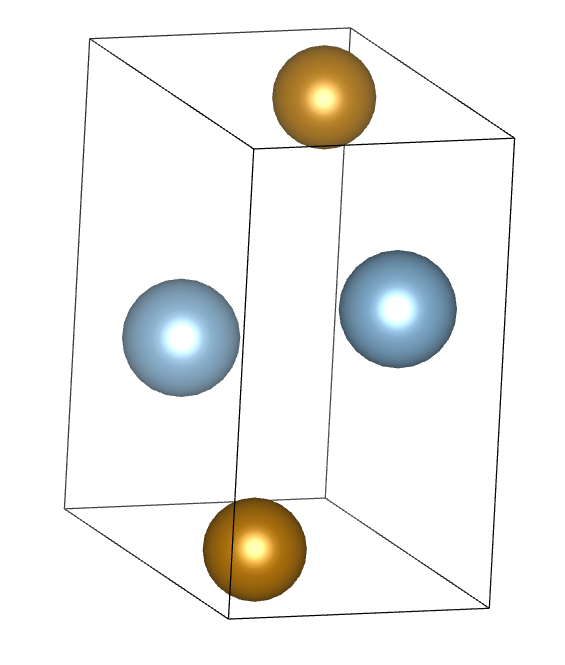
\includegraphics[width=0.30\textwidth]{content/cell.png}
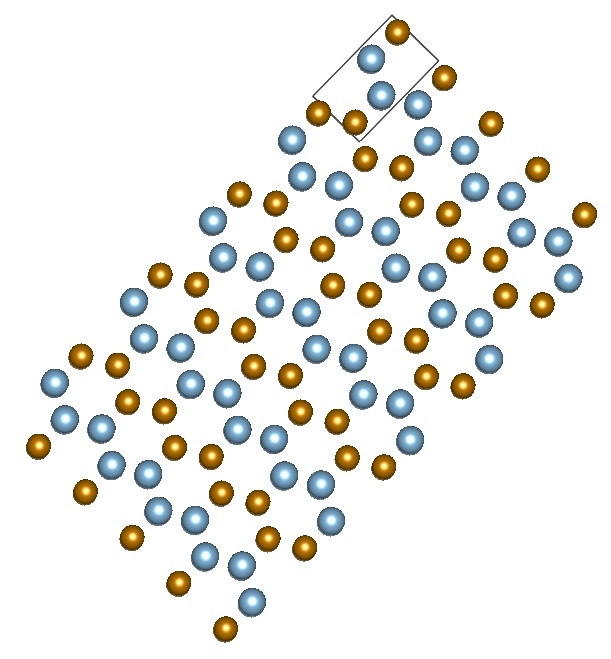
\includegraphics[width=0.30\textwidth]{content/ortho-1.jpg}
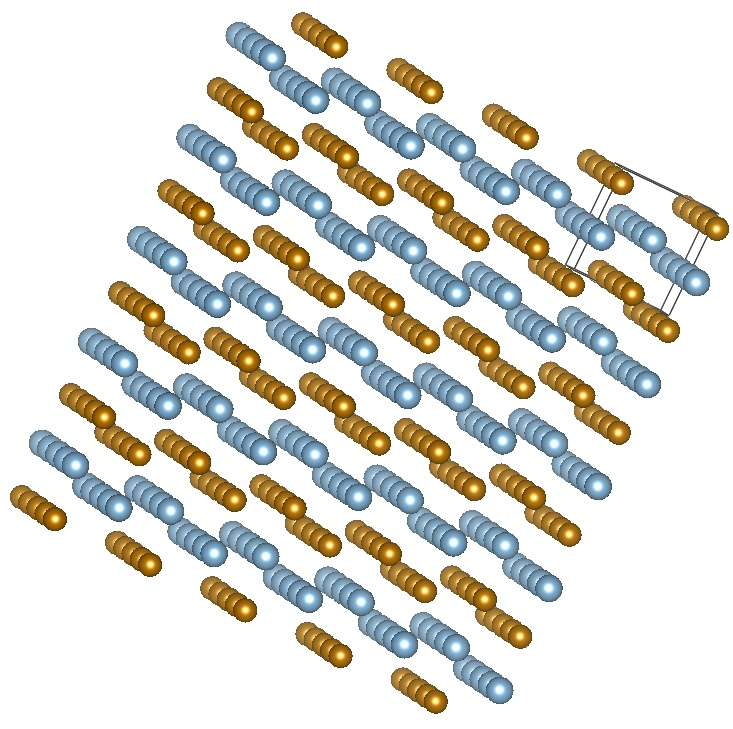
\includegraphics[width=0.30\textwidth]{content/ortho-2.jpg}
\caption{Views of the FeAl crystal and unit cell.}
\end{figure}

\section{Volume Optimization}
The unit cell was isotropically scaled to five volumes ($0.80$, $0.85$, $0.90$, $0.95$, and $1.00$ times the original $56.050$ \AA$^3$), and the total energy was computed at each volume with Quantum ESPRESSO (PBE PAW pseudopotentials, $E_{\text{cut}}^{\text{wfc}}=70$ Ry, $E_{\text{cut}}^{\rho}=700$ Ry, a $6\times4\times4$ $k$-mesh, Marzari-Vanderbilt smearing with $\sigma=0.005$ Ry, and an SCF convergence threshold of $10^{-8}$). The resulting $E$-$V$ points were fit to a Birch-Murnaghan equation of state using ASE's \texttt{EquationOfState} module, giving
\[
V_0 = 48.940 \text{\AA}^3, \qquad E_0 = -10034.793 \text{ eV}, \qquad B_0 = 170.55 \text{ GPa}.
\]
The optimized volume is about 12.7\% smaller than the nominal (unrelaxed) cell volume, indicating the as-given structure was not volume-relaxed at this level of theory.

\begin{figure}[H]
\centering

\includegraphics[width=0.6\textwidth]{content/eos_fit.png}
\caption{Birch-Murnaghan equation of state fit to the $E$-$V$ data.}
\end{figure}

\section{Cell Shape Optimization}
Cell shape optimization was performed on the ratio $\frac{b}{a}$, keeping the ratio $\frac{c}{a}$ fixed at its original value, $c/a=1.7320$, and the volume fixed at the optimized value from Section 1, $V_0=48.940$ \AA$^3$. For each of eight target $b/a$ ratios (the original ratio $b_0/a_0=1.6330$ scaled by factors of $0.97$ to $1.04$), $a$, $b$, and $c$ were solved for analytically to satisfy $abc=V_0$ at the fixed $c/a$, and an SCF energy was computed at each point with the same medium-precision settings as Section 1.

\begin{figure}[H]
\centering
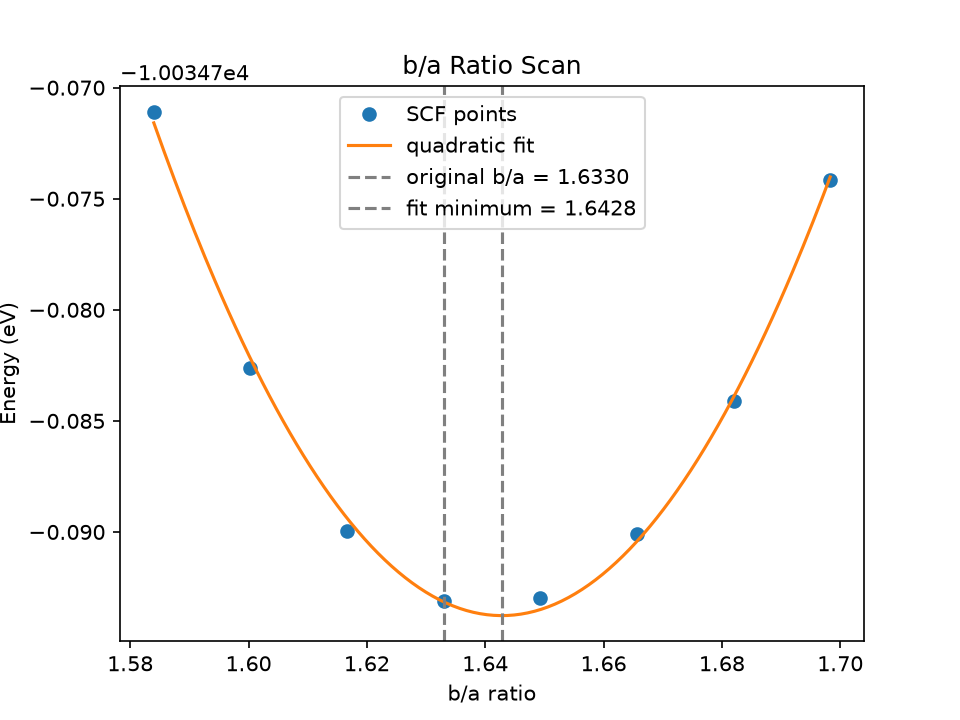
\includegraphics[width=0.6\textwidth]{content/ratio_quadratic_fit.png}
\caption{Energy versus $b/a$ ratio at fixed volume $V_0$ and $c/a$.}
\end{figure}

A quadratic fit to the eight points gives a minimum at $b/a \approx 1.6428$, only $0.6$ meV below the energy at $b_0/a_0=1.6330$, itself the lowest-energy point sampled. The original $b/a$ and $c/a$ ratios are thus already close to optimal once the volume is relaxed, and the energy scale here is $\approx 1$ order of magnitude smaller than for the volume optimization---the shape dependence is much weaker.

Rebuilding the cell at this ratio (again fixing $c/a=1.7320$ and $abc=V_0$) gives the optimized lattice lengths
\[
a = 2.5813 \text{\AA}, \qquad b = 4.2406 \text{\AA}, \qquad c = 4.4709 \text{\AA} \qquad (V=48.940 \text{\AA}^3),
\]
which, with atoms still at their original fractional coordinates, is carried into the position relaxation in Section 3.

\section{Atomic Position Relaxation}
Every calculation so far used a rigid \texttt{scf} run, so Fe (Wyckoff $2a$) and Al ($2b$) remained at their ideal, as-given free-parameter values, $z_{\text{Fe}}=0.91667$ and $z_{\text{Al}}=0.41667$. A \texttt{relax} calculation (fixed cell, \texttt{ion\_dynamics = bfgs}) was run on the Section 2 cell to find the true equilibrium positions, using $E_{\text{cut}}^{\text{wfc}}=70$ Ry, $E_{\text{cut}}^{\rho}=700$ Ry, a $6\times4\times4$ $k$-mesh, Marzari-Vanderbilt smearing with $\sigma=0.005$ Ry, and a $10^{-9}$ SCF threshold.

BFGS converged in 7 ionic steps (8 SCF cycles), lowering the total force from $0.034$ to $0.001$ Ry/bohr and the total energy from $-10034.793766$ eV to $-10034.876663$ eV, a further $82.9$ meV.

Site symmetry pins the $x$ and $y$ coordinates of all four atoms; only the free $z$ parameter relaxed:
\[
z_{\text{Fe}}: \ 0.91667 \rightarrow 0.90248 \ (\Delta z = -0.0142,\ -0.063 \text{\AA}),
\]
\[
z_{\text{Al}}: \ 0.41667 \rightarrow 0.39418 \ (\Delta z = -0.0225,\ -0.101 \text{\AA}).
\]
Each symmetry-related partner site shifts by the same amount in the opposite direction, being fixed at $1-z$. Al displaces about $60\%$ further than Fe.

\section{Full Optimization (vc-relax)}
Sections 1--3 optimized volume, shape, and positions one at a time, each holding the other degrees of freedom fixed. To relax all of them simultaneously, a \texttt{vc-relax} calculation was run starting from the Section 3 relaxed structure, at higher precision ($E_{\text{cut}}^{\text{wfc}}=90$ Ry, $E_{\text{cut}}^{\rho}=900$ Ry, a $14\times8\times8$ $k$-mesh, $10^{-9}$ SCF threshold).

BFGS converged in 10 ionic steps (11 SCF cycles), meeting all three criteria: energy change $<10^{-4}$ Ry, max.\ force $<10^{-3}$ Ry/bohr, and cell gradient error $<0.5$ kbar (reached $0.44$ kbar, with the trajectory pressure at that step $P=0.14$ kbar, down from $-3.2$ kbar initially). A separate, higher-accuracy static recalculation at the converged geometry---not itself subject to the convergence check---reports $P=1.07$ kbar; given $B_0=170.55$ GPa, this residual corresponds to a further volume change of only $\Delta V/V\approx P/B_0\approx6\times10^{-4}$, well below other sources of numerical error in the calculation. The total energy dropped further, from $-10034.876663$ eV to $-10035.141158$ eV ($-264.5$ meV). The cell remained orthorhombic (no shear developed), but its shape changed substantially even though the volume barely moved:
\[
a: 2.5813 \rightarrow 2.7416 \text{\AA} \ (+6.2\%), \quad b: 4.2406 \rightarrow 4.2420 \text{\AA} \ (\approx 0\%), \quad c: 4.4709 \rightarrow 4.1890 \text{\AA} \ (-6.3\%),
\]
\[
V: 48.940 \rightarrow 48.718 \text{\AA}^3 \ (-0.45\%), \qquad b/a: 1.6428 \rightarrow 1.5473, \qquad c/a: 1.7320 \rightarrow 1.5279.
\]
So the $c/a=1.7320$ constraint held fixed throughout Sections 2--3 was, in fact, far from the true equilibrium---only the volume and $b/a$ ratio had actually been optimized.

The $x$ and $y$ coordinates remained pinned by symmetry. Notably, the $z$ parameters relaxed back toward their original, ideal values once the cell was free to move with them:
\[
z_{\text{Fe}}: \ 0.90248 \rightarrow 0.91984 \ (\text{original: } 0.91667), \qquad z_{\text{Al}}: \ 0.39418 \rightarrow 0.41550 \ (\text{original: } 0.41667).
\]
This suggests the sizable $z$-shifts found in Section 3 were largely an artifact of relaxing positions inside a cell shape that was not itself at equilibrium, rather than a real deviation from the ideal HCP structure.

\end{document}
